\documentclass{beamer}

\usepackage[utf8]{inputenc}
\usepackage[english]{babel}
\usepackage{textpos}
\usepackage{graphicx}
\usepackage{textcomp}
\usepackage{animate}
\usepackage{comment}
%\usepackage{multicol}
%\setlength{\columnsep}{5cm}
\usepackage{amsmath}
\usepackage{amsfonts}
\usepackage{verbatim}
\usepackage{varwidth}
\usepackage{caption}
\usepackage{dcolumn}
\usepackage{amssymb}
\usepackage{algorithm}
\usepackage{algorithmic}
%\usepackage{physics}
\usepackage{hyperref}
\usepackage{scalerel,stackengine}
%\usepackage{fancyvrb}
%\usepackage{enumitem}
\usepackage{tikz}
\usepackage{pgfplots}

%\setbeamertemplate{itemize items}[circle]
%\setbeamertemplate{itemize subitem}[square]

\usefonttheme[onlymath]{serif}

\newcommand{\code}[1]{\texttt{#1}}
\newcommand{\shp}{$>>>$ }
\newcommand{\tab}{\hspace*{22pt}}

\usetheme{Madrid}

\title{NumPy and Matplotlib}
\author{EEC 3150}
\date{}

\institute{Trevecca Nazarene University}
 


%%%%%%%%% BEGIN DOCUMENT %%%%%%%%%
%%%%%%%%% BEGIN DOCUMENT %%%%%%%%%
%%%%%%%%% BEGIN DOCUMENT %%%%%%%%%

\begin{document}

% get title page 
\frame{\titlepage}
 
%%%%%%%%%%
%%%%%%%%%%
\begin{frame}	
	\frametitle{Outline}
	\tableofcontents	
\end{frame}


%%%%%%%%%%
%%%%%%%%%%
\section{Gradient Descent}

\begin{frame}	
	\center{\Huge{Gradient Descent}}
\end{frame}

\begin{frame}	
	\frametitle{Gradient Descent}
	
	\begin{alertblock}{Optimization:}
		\textbf{Optimization} is the process of finding the minimum/maximum value of a function $f(x)$ over some domain $D$:
		
		\vspace{5pt}
		\minipage{0.5\textwidth}
			\begin{equation*}
				\min_{x \in D} f(x)
			\end{equation*}
		\endminipage\hfill
		\minipage{0.5\textwidth}
			\begin{equation*}
				\max_{x \in D} f(x)
			\end{equation*}			
		\endminipage\hfill
		
		\vspace{10pt}
		\begin{itemize}
			\item $f$ is called the \textbf{objective function}
			\item $D$ is called the search space
			\item A value of $x$ which minimizes/maximizes $f$ is called a minimum/maximum (more generally, extremum)
		\end{itemize}
	\end{alertblock}
\end{frame}

\begin{frame}	
	\frametitle{Random Walks}
	
	\begin{block}{Applications of optimization:}
		\begin{itemize}
		\item Engineering: used in computer-aided design (e.g., finding the ideal plane wing to minimize drag but maximize lift)
		\item Physics: used to fit models of physical systems to observed data (my research!)
		\item Machine learning: used to train models (e.g., minimizing the loss function in neural networks)
		\item Operations research: used to solve problems in logistics, resource allocation, scheduling, and other areas of business and industry
		\item Finance: used to optimize investment portfolios and manage risk
		\item Game theory: used to model and analyze strategic interactions between agents
		\end{itemize}
	\end{block}
	
\end{frame}

\begin{frame}	
	\frametitle{Random Walks}
	
	\minipage{0.48\textwidth}
		\begin{alertblock}{Global vs. local:}
			\footnotesize
			\begin{itemize}
				\item A \textbf{global minimum} is a value $x^*$ such that $f(x^*) \le f(x)$ for all $x \in D$
				\item A \textbf{local minimum} is a value $x^*$ such that $f(x^*) \le f(x)$ for all $x$ in a neighborhood of $x^*$ (meets the calculus criteria for extremum, but isn't an extremal value)
			\end{itemize}
		\end{alertblock}
	\endminipage\hfill
	\minipage{0.02\textwidth}
		% blank
	\endminipage\hfill
	\minipage{0.48\textwidth}
		\begin{center}
			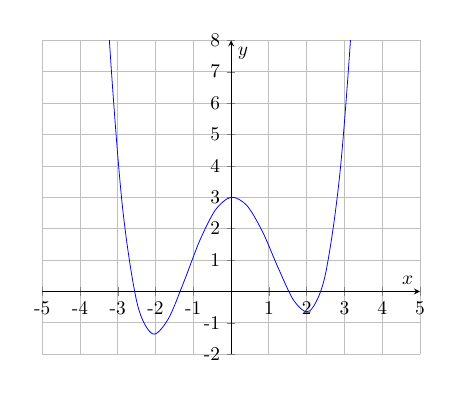
\begin{tikzpicture}[scale=0.7]
			\begin{axis}[
			axis lines=middle,
			xmin=-5,
			xmax=5,
			ymin=-2,
			ymax=8,
			xlabel=$x$,
			ylabel=$y$,
			xtick={-5,-4,-3,-2,-1,0,1,2,3,4,5},
			ytick={-2,-1,0,1,2,3,4,5,6,7,8},
			xticklabels={-5,-4,-3,-2,-1,0,1,2,3,4,5},
			yticklabels={-2,-1,0,1,2,3,4,5,6,7,8},
			grid=both
			]
			\addplot[domain=-5:5,smooth,blue] {(0.7*x)^4 - 4*(0.7*x)^2 + 0.25*(0.7*x) + 3};
%			\draw[dashed] (2,-2) -- (2,8);
%			\node[above right] at (2,7.5) {local minimum};
%			\node[below right] at (2,-2) {global minimum};
			\end{axis}
			\end{tikzpicture}
		\end{center}
	\endminipage\hfill
	
\end{frame}

\begin{frame}
	\frametitle{Optimization}
	
	\begin{alertblock}{Gradient descent (GD):}
		\footnotesize
		\begin{itemize}
			\item Gradient descent is an optimization method which uses the gradient/derivate of a function to find its minimum
			\item Given a starting point ($x_0$), it iteratively generates points by traveling along the direction of the function's steepest descent, i.e., the negative of the gradient
			\item The learning rate $\alpha$ (usually less than 1) controls the speed of descent
		\end{itemize}
	\end{alertblock}
	
	\begin{algorithm}[H]
		\caption{Gradient descent}
		\begin{algorithmic}[1]
			\STATE Set: learning rate $\alpha$, number of iterations $N$
			\STATE Set: $x_0$
			\FOR{$i=0$ to $N-1$}
				\STATE $x_{i+1} = x_i - \alpha \nabla f(x_i)$
			\ENDFOR
			\STATE Return: $x_N$
		\end{algorithmic}
	\end{algorithm}

\end{frame}

\begin{frame}
	\frametitle{Optimization}
	
	\begin{block}{Problems with gradient descent:}
%		\footnotesize
		Gradient descent is one of the simplest optimization methods and, thus, has many shortcomings:
		\begin{itemize}
			\item It can get stuck in local minima
			\item It can oscillate b/t solutions
			\item Gradients can explode
		\end{itemize}
	\end{block}

\end{frame}


%%%%%%%%%%
%%%%%%%%%%
\section{Simulated Annealing}

\begin{frame}	
	\center{\Huge{Simulated Annealing}}
\end{frame}

\begin{frame}
	\frametitle{Simulated Annealing}
	
	\begin{alertblock}{Simulated annealing (SA):}
		\footnotesize
		\begin{itemize}
			\item Simulated annealing is a more robust optimization method that is immune to many of the pitfalls of gradient descent
			\item It is based on the metalurgical process of annealing, where a metal is heated to a high temperature and then cooled slowly, causing it to become stronger by allowing the molecules in it to find a more optimal, low-energy state
			\item Given a starting point ($x_0$), it randomly generates potentially better candidate solutions from a probability distribution (usually a normal centered on the current solution)
			\item If the candidate solution is better than the current solution, accept it
			\item If the candidate solution is worse than the current solution, maybe accept it or not (depending on how much worse it is)
			\item This helps prevent SA from getting stuck in local minima
			\item As the method runs, it becomes pickier about accepting worse solutions
		\end{itemize}
	\end{alertblock}

\end{frame}

\begin{frame}
	\frametitle{Simulated Annealing}
	
	\begin{block}{Some terms:}
		\begin{itemize}
			\item Proposal distribution $q(x',x_i)$: the distribution from which new candidate solutions $x'$ are drawn \\
			Example: normal distribution centered on the current solution $x_i$ \\
			Proposal width: the stddev of the normal
			\item Cooling schedule: the function which defines the rate at which the ``temperature'' decreases \\
			Example: $T_i = T_0 \exp( -i / \tau )$
			\item Acceptance probability $\alpha(x',x_i)$: the probability that a candidate solution will be accepted
		\end{itemize}
	\end{block}
	
\end{frame}

\begin{frame}
	\frametitle{Simulated Annealing}
	
	\begin{algorithm}[H]
		\caption{Simulated Annealing}
		\begin{algorithmic}[1]
			\STATE Set: number of iterations $N$, cooling schedule 
			\STATE Set: $x_0$
			\FOR{ $i=0$ \TO $N-1$}
				\STATE Generate new candidate \\ $x' \sim q(x',x_{i})$
				\STATE Calculate change in function value \\ $\Delta f = f(x') - f(x_i)$
				\IF{ $\Delta f<0$ }
					\STATE Accept candidate \\ $x_{i+1} = x'$
				\ELSE
					\STATE Accept candidate w/ probability $\alpha(x',x_i) = \exp(-\Delta f / T_i)$ \\
					Either $x_{i+1} = x'$ or $x_{i+1} = x_i$
				\ENDIF
			\ENDFOR
		\end{algorithmic}
	\end{algorithm}

\end{frame}

\begin{frame}
	\frametitle{Optimization}
	
	\begin{block}{Problems with simulated annealing:}
%		\footnotesize
		Though SA addresses some of the issues with GD, it is still imperfect:
		\begin{itemize}
			\item It usually converges slowly
			\item Requires parameter tuning/adaptation
			\item Can still get stuck in local minima, but not nearly as badly as GD
		\end{itemize}
	\end{block}

\end{frame}

\begin{frame}
	\frametitle{Optimization}
	
	\begin{exampleblock}{:}
%		\footnotesize
		Though SA addresses some of the issues with GD, it is still imperfect:
		\begin{itemize}
			\item It usually converges slowly
			\item Requires parameter tuning/adaptation
			\item Can still get stuck in local minima, but not nearly as badly as GD
		\end{itemize}
	\end{exampleblock}

\end{frame}

\begin{frame}	
	\frametitle{Monte Carlo Simulation}
	
	\begin{exampleblock}{Calculate statistics of a complex distribution:}
		\small
		A cannon can fire a cannonball with an initial velocity $v_i$ at an angle $\theta$
		\begin{align*}
			x_f & = x_i + v_i \cos(\theta) t \\
			y_f & = y_i + v_i \sin(\theta) t - \frac{1}{2}gt^2
		\end{align*}
		
		Assuming that the cannon can only launch the ball at $vi = 100$ m/s, use simulated annealing to determine what angle the cannon must be aimed to hit a target $\hat x_f=500$ m away \\[10pt]
		
		Model ($x_i,y_i,y_f = 0$): \\[-20pt]
		\begin{align*}
			x_f(\theta) = \dfrac{v_i^2 \sin(2\theta)}{g}
		\end{align*}
				
		Objective function (squared error): \\[-20pt]
		\begin{align*}
			f(\theta) & = \Big(\hat x_f - x_f(\theta)\Big)^2
		\end{align*}
	\end{exampleblock}
	
\end{frame}


\end{document}




